\end{multicols}
\newpage
\subsection{Studentische Selbstverwaltung f"ur Dummies}

  \ifpdf
    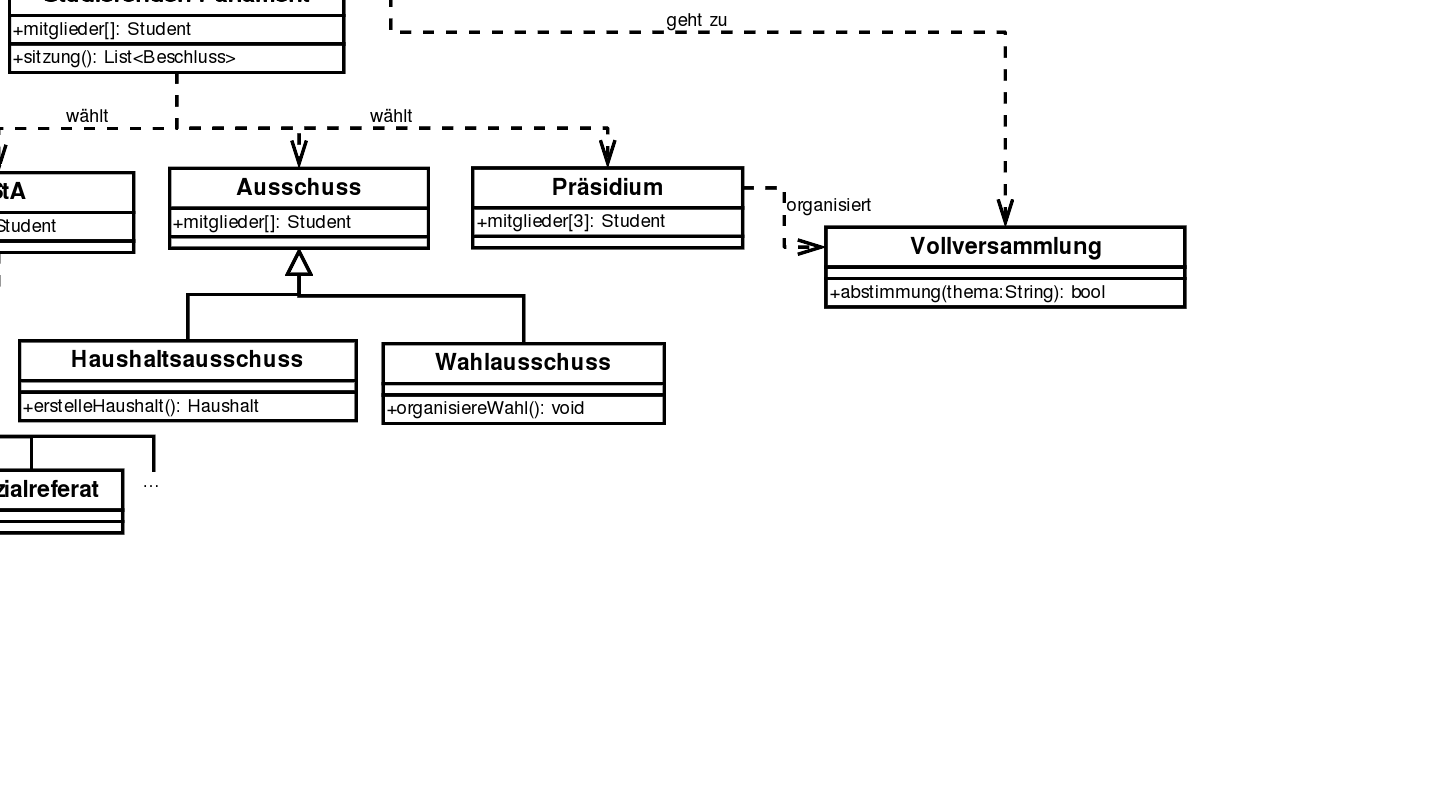
\includegraphics[width=\textwidth]{bilder/gremienkunde2.png}
  \else
    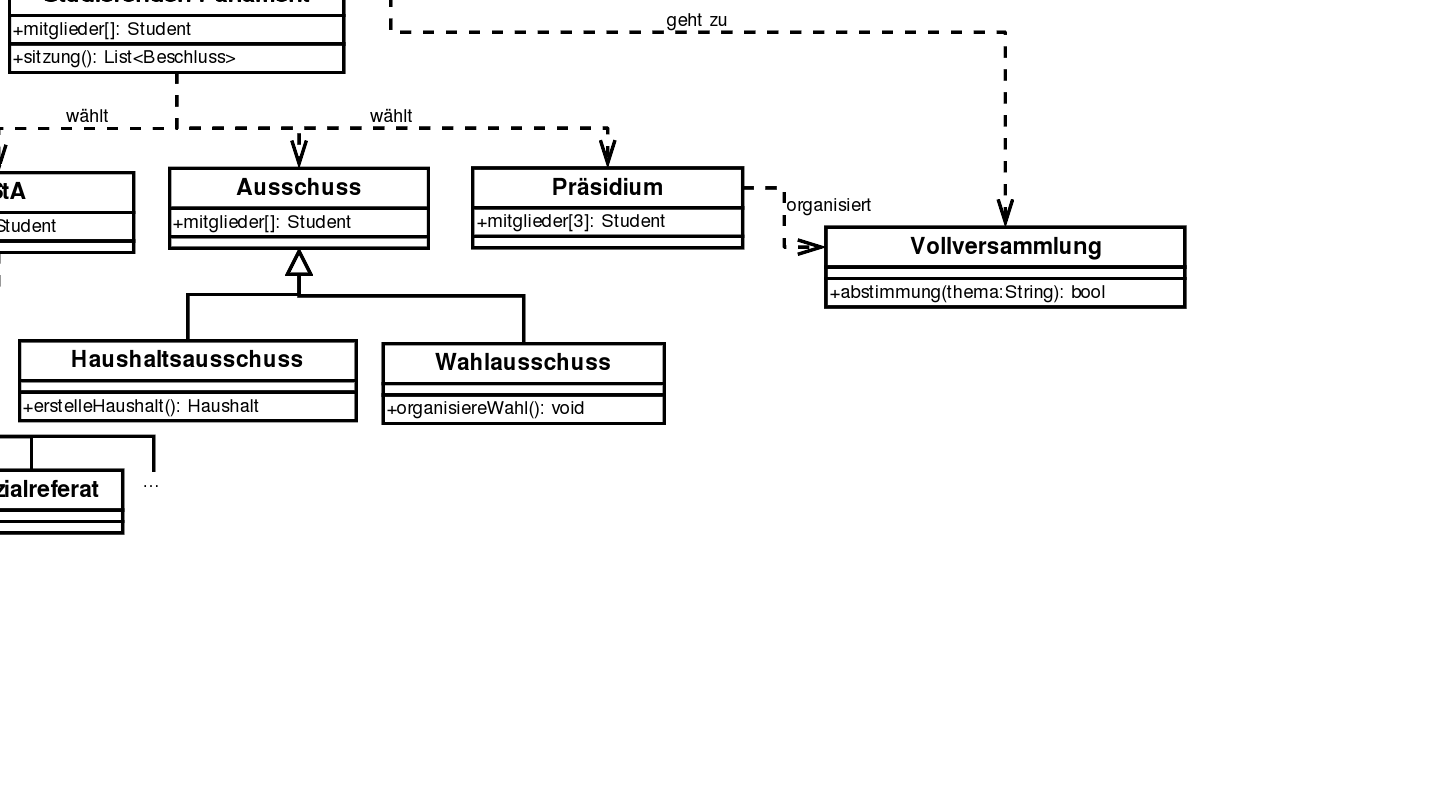
\includegraphics[width=\textwidth]{bilder/gremienkunde2.png}
  \fi
\begin{multicols}{2}
Seit die '68er durch die deutschen Universit"aten gefegt sind, 
ist Demokratie eingekehrt.
Doch was bedeutet das konkret f"ur euch?

\subsubsection*{Studierendenparlament}
Eines der wichtigsten Elemente der studentischen Mitbestimmung 
ist das Studierendenparlament (Uni-Slang: StuPa).
Es wird jedes Semester gew"ahlt und entscheidet unter anderem 
"uber den studentischen Haushalt, den ihr als Teil des Semesterbeitrags 
zahlt. Au"serdem werden hier Aussch"usse gew"ahlt (Als wichtigster 
der "`Allgemeine Studierenden Ausschuss"', kurz AStA).

\subsubsection*{AStA}
Der Allgemeine Studierenden Ausschuss ist die "`Exekutive"' der 
Studenten: Er vertritt euch nach Au"sen, also zum Beispiel bei 
Verhandlungen um das Semesterticket, versorgt euch mit Informationen 
zu politischen Themen ("ofter im Semester erscheint der so genannte 
"`AStA-Issue"') und ist einer der ersten Ansprechpartner f"ur eure 
Anliegen.

\subsubsection*{Fachgruppe}
Auch die Fachgruppe wird von euch gew"ahlt.
Allerdings w"ahlt hier jede Fachrichtung ihre eigene, ihr also 
Fachgruppe Informatik. Die Fachgruppe unterst"utzt euch bei 
Infomatik-spezifischen Fragen, organisiert Veranstaltungen, wie zum 
Beispiel eure Erstsemester-Einf"uhrung und vertritt euch in 
verschiedenen Gremien.

\subsubsection*{Gremien}
In der Uni gibt es unz"ahlige Gremien, hier seien die wichtigsten
genannt. Jedes Gremium hat eine bestimmte Besetzung, also eine 
definierte Anzahl von jeweils Studenten, Mitarbeitern und Professoren.
Am relevantesten für euch ist die Studienkommission (\emph{StuKo}):
Hier werden Details des Studiengangs besprochen, Probleme der 
Studenten gekl"art und die Vergabe der Studiengebühren entschieden.
In diesem Gremium herrscht ein Stimmengleichgewicht zwischen 
Studenten und Professoren. Das bedeutet, dass wir hier wirklich 
die M"oglichkeit haben, aktiv in die Unipolitik einzugreifen.

In der \emph{Informatik-Kommission} und im \emph{Fakult"atsrat} 
(der au"serdem noch Mitglieder aus der Mathematik hat) sieht es da 
schon schlechter aus, die Studenten stellen in beiden nur eine 
Minderheit der Stimmen.

Die \emph{Berufungskommission} hat nur selten zu tun:
Wann immer eine Professur besetzt werden muss, tagt sie um 
Kandidaten f"ur das Amt zu finden.

Wann immer ihr Antr"age im Pr"ufungsamt stellt, landen diese 
im \emph{Pr"ufungsausschuss}, der entscheidet, ob diese rechtm"a"sig 
sind. In diesem sind drei Professoren, ein Student und ein 
Mitarbeiter vertreten.

\subsection*{Vollversammlung}
Mindestens einmal im Semester findet eine Vollversammlung aller 
Studenten statt.
Nehmen genug Studenten teil, so k"onnen hier wichtige Themen 
abgestimmt werden, die alle Studenten betreffen, zum Beispiel 
wurde die Einf"uhrung des Semestertickets hier beschlossen.
Wenn ihr informiert darüber bleiben wollt, was neben eurem 
Studiengang so an der Uni vor sich geht, solltet ihr diese 
Versammlungen nicht verpassen.